\chapter{Design and Specification}

\section{Overview of System Architecture}

\begin{figure}[!ht]
    \centering
    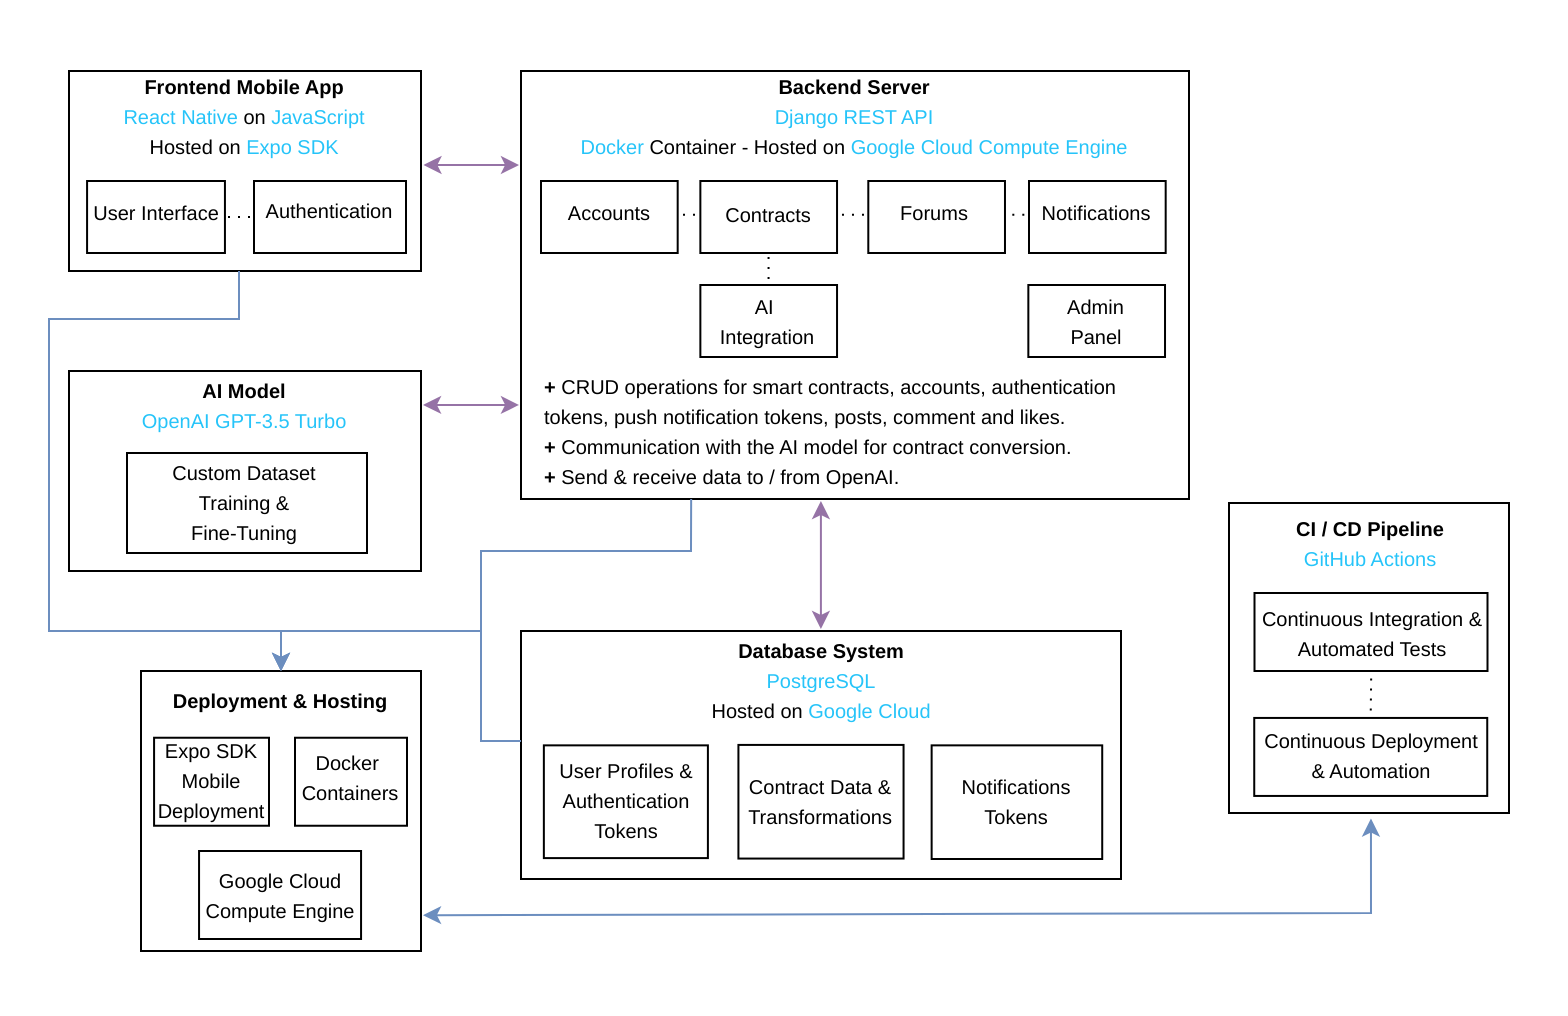
\includegraphics[width=1\linewidth]{LATEX/Appendices/Images/Software/software-diagram.png}
    \caption{Software Diagram}
    \label{fig:software-diagram}
\end{figure}

The platform will use Generative AI and smart contracts to address issues of automation and security in employment contracts. This will be achieved through fine-tuning \texttt{OpenAI's GPT-3.5 Turbo} model on a custom dataset to train it to convert legal employment contracts into smart ones. The backend server will be based on \texttt{Django Rest API} to handle data processing and interactions with the AI model. Apart from that, the mobile application interface will be built with \texttt{React Native on JavaScript}.

\section{Requirements and Objectives}

In order to successfully implement the platform, several requirements and objectives must be met. These needs can be divided into functional and non-functional categories.

\subsection{Functional Requirements}

Functional requirements specify the behaviours and features that the platform must exhibit in order to satisfy user demands and project objectives. Amongst them are:

\begin{itemize}
    \item \textbf{Contract Conversion:} The platform must be able to convert traditional employment contracts into smart contracts using the fine-tuned \texttt{GPT-3.5 Turbo} model.
    \item \textbf{AI Model Integration:} The AI model must be integrated into the backend, allowing for efficient processing of contracts.
    \item \textbf{User Authentication:} Users (employers and employees) must be able to securely create and manage their accounts.
    \item \textbf{User engagement:} The platform must provide a forum for users to interact with one another on topics related to the application's scope.
    \item \textbf{Contract Management:} Users must be able to create, view, update, and delete their smart contracts.
    \item \textbf{Performance Metrics:} The platform should support the input and management of performance metrics relevant to various job roles, which can later be expanded to automatic updates from the backend.
    \item \textbf{Salary Management:} The system must handle salary payments using \textit{USDC Coin}.
    \item \textbf{Notifications:} The platform must send notifications to users regarding contract updates, salary payments, and other relevant events.
    \item \textbf{Mobile Application:} The mobile application must provide a user-friendly interface for both iOS and Android users to interact with the platform's features.
    \item \textbf{Custom Theming:} The user interface (UI) should support dark and light modes.
    \item \textbf{Admin Panel:} The backend must include an admin panel for managing users, contracts, and system settings efficiently.
    \item \textbf{Dispute Resolution:} The platform should provide mechanisms for resolving disputes between employers and employees based on contract terms.
\end{itemize}

\subsection{Non-Functional Requirements}

Non-functional requirements verify that the platform operates efficiently and reliably. These include:

\begin{itemize}
    \item \textbf{Scalability:} The system must be able to handle an increasing number of users and contracts without performance degradation.
    \item \textbf{Security:} The platform must securely handle data, especially those concerning financial transactions and sensitive contract details. This includes secure authentication and regular audits.
    \item \textbf{Reliability:} The platform must be highly reliable, with minimal downtime, to ensure users can access and manage contracts whenever needed.
    \item \textbf{Performance:} The system must provide quick response times for user interactions, contract processing, and AI model predictions.
    \item \textbf{Usability:} The mobile application interface must be intuitive to provide a positive user experience.
    \item \textbf{Compliance:} The platform must comply with relevant regulations regarding employment contracts and data protection.
    \item \textbf{Maintainability:} The codebase should be modular and well-documented, allowing for easy maintenance and future updates.
    \item \textbf{Portability:} The system should be deployed across various environments through cloud services with minimal configuration changes.
\end{itemize}

\section{Conceptual Development and Methodological Shifts}

\subsection{Rationale Behind Architectural Choices}

The decisions on architecture were based on the needs for efficiency, scalability, and robustness. Every component of the platform has been picked to maximise the output of the functionality, simultaneously providing a good user experience.

\subsection{AI Model Selection}

\begin{itemize}
    \item \textbf{Hugging Face Models:} Selecting the appropriate AI model for fine-tuning was one of the most important early decisions to make. Initially, it was planned to take a \texttt{seq2seq} transformer model from \textit{HuggingFace} and train it through \textit{PyTorch} framework. However, upon further investigation, it became clear that the vast majority of available models there were based on the \textit{GPT} architecture ranging from version \textit{2.0} to \textit{3.0} \cite{GerstmayrEtAl2024, Campesato2023}. Although these variations are quite effective, they are still worse than more modern ones. Moreover, \textit{HuggingFace} itself suffers from multiple limitations, including the challenge of context-dependent model selection \cite{NarayananEtAl2023}. With over 262,000 models available, users face the daunting task of choosing the optimal model for specific workflows or data domains, complicated by the wide variety of model architectures, sizes, and training paradigms \cite{Jones2024, NarayananEtAl2023}. Additionally, different models exhibit variable performance across tasks and datasets, meaning that a model excelling in one area may not be suitable for another, necessitating extensive testing and customisation \cite{NarayananEtAl2023, Campesato2023}. Yet, for the sake of exploring possible options, it was attempted to fine-tune two models from the platform: \textit{Salesforce/codegen-350M-multi} and \textit{EleutherAI/gpt-neo-125m}. Nonetheless, no significant results have been achieved, as the models were not generalising properly. This was most likely because of the architecture limitations \cite{LucianoEtAl2020}, such as a lack of contextual awareness, inability to fully understand complex contractual terms, and challenges in generating syntactically correct \textit{Solidity} code. To be more precise, these models struggled the most with the translation of elements like wallet addresses and transactional clauses. No mistakes can be tolerated here since, if the model interprets an address wrongly, this would result in financial losses. Consequently, this led to the exploration of other models unrelated to \textit{HuggingFace}, bringing us to \textit{OpenAI}. 
    \item \textbf{OpenAI Models:} While investigating \textit{OpenAI} further, it became apparent that they allow for fine-tuning one of the latest models, \texttt{GPT-3.5 Turbo}. The process simply requires the provision of custom datasets for training and validation \cite{LatifEtAl2024, OpenAIDocumentation2023}. A \textit{GPU} is not needed since the model gets trained on \textit{OpenAI's} servers \cite{ChatGPTFineTuning2024, OpenAIDocumentation2023}. Moreover, \textit{HuggingFace} models require manually writing the training algorithm. This includes tokenisation logic with appropriate padding and encoding, selecting the appropriate batch sizes, setting up warm-up steps, weight decays, and evaluation strategies \cite{NarayananEtAl2023}. The problem is, it is hard to select the best figures, and to do so, one needs a deep knowledge of how transformers work. On the contrary, \textit{OpenAI} does not require these patterns to be specified, as they automatically choose the best options for each specific case through permutations during the training process \cite{OpenAIDocumentation2023}. This has further highlighted the advantage of OpenAI's solution.
\end{itemize}

Summarising, this model was chosen because of its advanced natural language processing capabilities compared to earlier versions of that transformer, such as \textit{GPT-2.0}. The \textit{GPT-3.5 Turbo} model is financially practical, given the ratio of cost to performance. However, it is worth noting that at the time of the design phase, the \textit{GPT-4.0} model was not yet available for fine-tuning, limiting the choice to the existing models. Moreover, other options from \textit{HuggingFace} were considered and implemented; however, they neither scaled properly nor generalised effectively in terms of handling large volumes of queries without degradation in response times or accuracy. This led us to ultimately settle on \textit{OpenAI's} solution.  
        
\subsection{Selection of Backend and Frontend Frameworks}

At the beginning of the project, it was planned to use Flask for the backend and native development for the mobile interface. Flask, a simple Python web framework, seemed like a good choice because of its simplicity. It was also considered to implement separate Android and iOS interfaces to take advantage of the platform-specific features. However, moving forward, it was realised that these choices had some drawbacks:

\begin{itemize}
    \item \textbf{Scalability Concerns with Flask:} Starting with Flask was a good idea at first, but concerns arose regarding its scalability and its ability to efficiently handle the complex data processing \cite{Ghimire2020, CopperwaiteEtAl2015} required by the AI and smart contract components as the project grew.
    \item \textbf{Duplication of Efforts in Native Development:} Developing separate native applications for \texttt{Android} and \texttt{iOS} would have meant doubled effort, increased development time, and challenges in maintaining code consistency across platforms \cite{MasielloEtAl2017}.
\end{itemize}

These findings led to a change towards Django Rest API and React Native. The rationale behind this shift was multi-faceted:

% addd citations here for hte other frameworks %
\begin{itemize}
    \item \textbf{Django Rest API:} This framework offers time-proven robustness, which arises from the large amount of existing built-in functionalities and community support \cite{HillarEtAl2018}. Apart from that, it is well-documented, secure and reliable \cite{Ghimire2020, HillarEtAl2018}. Moreover, the framework itself is relatively easy in terms of syntax, and the entry threshold is quite low compared to other popular frameworks \cite{HillarEtAl2018, EliseevaEtAl2020, Plekhanova2009, Mao2018} such as \texttt{Ruby on Rails} \cite{LaurentEtAl2008}, \texttt{Node.js} \cite{Mead2018} and \texttt{ASP.NET} \cite{Ragupathi2016}. Additionally, it was chosen due to personal familiarity, which would significantly speed up the implementation phase. On top of that, the admin panel provided by it simplifies data management tasks \cite{HillarEtAl2018}. Last but not least, it was decided to progress with the \texttt{Django Rest API} option since \textit{Flask} is not providing many built-in functionalities, heavily relaying on third-party libraries \cite{ChanEtAl2019}. Summarising, \textit{Flask} is more suitable for lightweight web applications \cite{ChanEtAl2019}. 
    \item \textbf{React Native:} This framework was chosen primarily for its ability to maintain one codebase for \texttt{iOS} and \texttt{Android} platforms, significantly reducing development time \cite{MasielloEtAl2017}. Research shows that users tend to prefer mobile applications over websites for tasks that require regular interactions \cite{TurnerMcGrievyEtAl2016, TupikovskajaOmovieEtAl2015, AlmarashdehEtAL2019, Warcholinski2024}. Although it is worth admitting that the researches presented are more focused on mobile applications developed for healthcare and sales, they still indicate that user engagement with these is slightly better than with websites. Furthermore, the choice was also driven by the desire to learn this framework, as it is widely adopted nowadays. In addition to native development, alternatives like \texttt{Flutter} have been considered. However, the large community of \texttt{React Native} and its mature ecosystem \cite{Wu2018, Boduch2017} swayed the choice towards it. Another major factor was that \texttt{React Native} allows for integration with native components \cite{Boduch2017}, which is extremely important in our case as we need secure storage for smart contracts when they are passed to users. Lastly, as \texttt{React Native} is almost identical to \texttt{React} \cite{Boduch2017}, this means that as soon as the mobile application is developed, the platform can easily be extend by creating a website. And due to the similarities between these frameworks, learning one would allow for easier adaptation to the other.
\end{itemize}

These technologies were integrated to ensure the platform meets the current demands and adapts for future expansions. The choice of each component provides a robust foundation for the platform’s success if implemented properly.

\subsection{Database System Selection}

\texttt{PostgreSQL} was chosen as the main database for the platform because it met several important needs for the project. The data being managed includes authentication and notification tokens, account details, and extensive text content for legal employment contracts and their smart counterparts. This required a database that could handle large volumes of information quickly, scale properly, and manage text effectively.

\begin{itemize}
    \item One of the reasons \texttt{PostgreSQL} is so great at handling complex data with large volumes of text is its advanced indexing and full-text search features, making it an ideal solution for applications that need fast search and retrieval of large amounts of text data \cite{WorsleyEtAl2002}. Furthermore, it is overwhelmingly vital to keep up with the accuracy of transactional data while dealing with legal and contractual obligations. \textit{PostgreSQL} fully complies with the principles of atomicity, consistency, isolation, and durability \cite{JubaEtAl2015}. It thus provides a guarantee for the reliable processing of all transactions. Lastly, the ecosystem and community of \textit{PostgreSQL} are huge. Hence, there is a great volume of plugins, tools, and support \cite{FotacheEtAl2013} which will ease management, integration, and troubleshooting. 
    \item \textit{PostgreSQL} has the ability to function not only as a relational but also as a \texttt{NoSQL} database \cite{TruskowskiEtAl2020}. In contrast, many \textit{NoSQL} databases are highly scalable but may compromise on transactional integrity. \textit{PostgreSQL}, however, balances both. It can manage a large increase in data volume and many users at the same time with little drop in performance \cite{DouglasEtAl2003, TruskowskiEtAl2020, FotacheEtAl2013}. This is important for a platform that will grow and handle more employment contracts. Furthermore, \textit{NoSQL} databases can handle various data types, such as unstructured text, multimedia files, and large data blobs. Their schema-less design allows flexibility for changes in data structure \cite{FotacheEtAl2013}, which is helpful for applications with dynamic data forms. However, for this application, the main data types are structured text strings and numerical values for user and contract data. The relational database model of \textit{PostgreSQL} is more suitable for this purpose. It offers structured query capabilities and strong transaction support \cite{WorsleyEtAl2002, TruskowskiEtAl2020, FotacheEtAl2013}, which are crucial for consistent and reliable management of all application data interactions.
    \item Comparing it with \texttt{MS SQL Server}, we can conclude that the latter is a powerful database, but its licensing and operational costs are higher compared to \textit{PostgreSQL}, which is open-source \cite{TruskowskiEtAl2020, FotacheEtAl2013}. 
\end{itemize}

In summary, \textit{PostgreSQL} was chosen for its powerful data handling abilities, especially for complex and large text data. Its adherence to \textit{ACID} compliance ensures transactional integrity. Additionally, \textit{PostgreSQL} is cost-effective and flexible, making it a perfect fit for the project's long-term goals and scalability needs.

\subsection{Smart Contracts: Initial Idea}

The initial idea was to utilise an AI model for the purpose of converting legal employment contracts into smart ones, specifically varying based on the job role.

\begin{itemize}
    \item It was planned to train the AI model to incorporate precise job metrics for various professions at the time of translation. 
    \item For professions related to computer science, quality metrics such as the quantity and quality of commits, as well as adherence to deadlines, would have been considered. For simpler roles, such as waiter or barista, metrics would have included location tracking during work hours and sales volume from an employer's company Customer Relationship Management (CRM) database. Similarly, for salespeople, smart contracts would automatically get data on sales achievements from a CRM and use it in the contract. For teachers and lecturers, performance indicators would include the number of lectures given and student feedback. 
    \item Furthermore, to expand on these ideas, other jobs might use metrics like project completion rates for construction workers, resolution success rates for customer service roles, and adherence to treatment plans for healthcare professionals. 
\end{itemize}  

However, as the project developed, several important realisations came up.

\begin{itemize}
    \item The variety of job roles meant that each job needed its own specific metrics for performance evaluation. This created a very complex system for integrating and verifying these metrics. The main challenge was where these metrics came from — usually the CRM systems of the hiring companies. CRM systems are often very different in how they are set up and organised, which made the integration process much harder. For similar job roles, metrics might have different names in different systems, like salesAchievedEmployeeXYZ versus salesEmployeeXYZ.
    \item Addressing these challenges would require creating an AI that can understand and script data retrieval from different CRM databases. This is a very tough technical task. Questions came up about the type of data needed. Would it be just the schema of the CRM database, or would it need more detailed data sets that include real-time performance metrics?
    \item Given the wide range of potential job scenarios, the initial idea, while promising, turned out to be almost impossible to implement. It was more akin to a PhD-level research project than a bachelor's thesis. It needed a lot of development resources and more advanced AI capabilities than were possible within the given time and available resources.
\end{itemize}

This realisation led to refocusing the scope of the project towards developing a more generalised smart contract framework. It will not be as customised to each job's specific metrics, but it will still greatly improve transparency, security, and reliability in employment management.

\subsection{Refocusing the Scope of Smart Contracts}

The focus was shifted towards training a simpler AI model capable of producing more general smart contracts, concentrating on the most important functionalities of the system. This change aims to provide both employers and employees with trust in the system to follow through on their contract obligations without any issues.

\subsection{Smart Contracts Design}

\begin{itemize}
    \item The intention is to handle salaries using USDC Coin, a stable cryptocurrency known for its reliability coming from the fact it is backed by US dollars. This choice helps reduce the risks linked to cryptocurrency price fluctuations, ensuring that salary payments remain steady. USDC was chosen over other stablecoins such as USDT because it is considered the safest option, as the developers of the coin regularly perform open audits \cite{LyonsEtAl2023, VediaEtAl2023}.
    \item Once a contract is deployed, its internal state cannot be changed unless explicitly specified in the original code. Thus, it was decided to add an external modifier that allows the backend to interact with the contract post-deployment. This modifier is extremely important because essentially it shifts the responsibility of tracking job performance metrics from the smart contract itself to the backend system. This is a more appropriate design choice since performing heavy computations directly in smart contracts can be financially impractical \cite{Buterin2014}. This approach lets us focus on developing an AI model that can create generalised smart contracts for managing financial interactions between employers and employees, ensuring security for everyone involved. However, since the process of implementing job performance metrics counting by the backend is overly complex and could potentially take longer than expected, it might be postponed to a later stage.
    \item The contract will include wallet addresses of the employers and employees. This is to ensure that all transactions, whether salary payments or dispute resolutions, are executed between the correct parties.
    \item The smart contract will include features to manage the employment period. It will be possible to set start and end dates, keep track of the last salary payment date, and handle contract extensions or terminations through public functions triggered by the backend using the authorised modifier. This flexibility allows the contract to adjust to real-world employment situations.
    \item Initially, the contract will allow for basic input regarding performance scores and thresholds by the authorised app, e.g., the backend. In the future, these metrics are planned to be automatically updated by the backend using actual job performance data. 
    \item Several functions will be implemented to automate salary transfers, bonuses, and job terminations based on data sent from the backend to the smart contract. These functions will operate automatically to ensure that financial transactions, like paying salaries and bonuses, happen promptly.
\end{itemize}

A more in-depth implementation of this design will be discussed during the implementation phase in the next chapter. The decision to prioritise these basic elements was influenced by practical considerations such as feasibility and resource availability, given the complexities and the need for a dependable, tamper-proof system. This focused approach aims to establish a strong foundation for secure and efficient employment management using blockchain technology. It also lays the groundwork for future improvements that could include advanced data integration and performance metric calculations.

\section{Integration Strategy}

The integration strategy of the platform involves the following key components:

\begin{itemize}
    \item \textbf{AI Model Integration:} The trained AI model is hosted on \texttt{OpenAI's} servers. The backend communicates with it through the API provided by \textit{OpenAI} using a unique secret key. This allows the backend to send contract data to the trained AI model and receive back the processed output.
    \item \textbf{Backend:} Initially, it was planned to deploy the backend on the \texttt{AWS} platform, as it is one of the best available options at the moment. However, the downside of it is that the cost might be high. Hence, it was decided to proceed with \texttt{Google Cloud}, as it offers low-cost subscriptions. To implement this, the \textit{Google Compute Engine} platform will be leveraged, which is essentially a ``serverful'' host.
    \item \textbf{Database:} The backend also manages the \textit{PostgreSQL} database, which securely stores user profiles, various tokens for authentication / notifications handling, legal employment contracts, their smart contract transformations, and other pertinent data. The plan is to host it on \textit{Google Cloud Storage}, which is a reliable cloud-based storage solution.
    \item \textbf{Mobile Application:} The same problem was encountered with the frontend. Initially, it was intended to be deployed for both \textit{iOS} and \textit{Android} platforms on the \textit{Apple App Store} and \textit{Google Play Store}, respectively. However, the fees these platforms require are too high, and are justifiable for enterprise applications that generate revenue, not for academic projects. Hence, it was decided to proceed with \texttt{Expo's SDK}.
\end{itemize}